%!TEX root = main.tex

\chapter{Analysis of Eurocode criteria}

This chapter aims to analyze the Eurocode criteria that are related to lateral dynamics of railway bridges and discover their background principle. There are two types of criteria: bridge-natural frequency based criterion and vehicle-induced lateral force criterion. 

It has been discovered that UIC research\citep{d181} is the original research that proposed both types of criteria.

\section{Criterion based on bridge natural frequency}

\paragraph{Criterion definition and background}
The bridge natural frequency based criterion is defined in \citep[A24.4.2.4]{EC12} by following statement:

\begin{quote}
	...

	\emph{The first natural frequency of lateral vibration of a span should not be less than $f_{h0}$. The value for $f_{h0}$ may be defined in the National Annex. The recommended value is: $f_{h0}=1.2 Hz$}

	...
\end{quote}

The original proposal can be found in \citep[Proposed criteria]{d181}. The original intension of criterion is explained by following quote text:

\begin{quote}
	\emph{To avoid the occurrence of resonance in the lateral motion of the vehicles due to the lateral motion of the bridge, a limit value lower than the first natural frequency $f_1t$ of the lateral vibration of the span studied should be fixed. The natural frequency for lateral movements is between 0.5 and 0.7 Hz for coaches and between 0.7 and 1 Hz for locomotives. We therefore propose a safety margin $F_{lt} \geq 1.2Hz$}
\end{quote}

\paragraph{Criterion principle} From the original proposal, it can be concluded that this criterion intends to avoid the resonance between the vehicle and the bridge. 

There is no additional explanation about what type of resonance is being avoided. The \emph{natural frequency} in the original text is also unclear. There is no explanation on the natural frequency, either.  

It can be concluded that the original text is referring to the natural frequency of an uncertain vibrating mode of the vehicle. The magnitude of the frequency in original proposal is independent of speed, thus it can be guessed that the frequency refers to the natural frequency of a typical rigid body mode of the vehicle. It may be the lateral swing mode of railway vehicles.

However, the resonance described in the original text does not belong to any resonance type validated in previous research. This is because resonance caused by both axle repeat pattern and kinematic movement happens at frequencies related to vehicle speed. There is no research supports the resonance theory described in this criterion.

As a conclusion, the criterion lacks theoretical support. No evidence proofs the resonance mentioned in the original text can happen.  No background principle can be extracted from this criterion.

\section{Criterion based on vehicle-induced lateral force}
The criterion based on vehicle-induced lateral force is the global criterion governing the validation of structural safety. The criterion itself is generic and unrelated to the topic of lateral dynamics of railway bridge. To be more specific, this section aims to analyze the vehicle-induced lateral force which is a load input for the global criterion.

There are several types of vehicle-induced lateral force mention in Eurocode\citep{EC12} but this thesis only concerns uniform motion and straight railway tracks. Thus one type of force, Nosing force, is selected and analyzed. 

\paragraph{Definition and background of nosing force} 
The nosing force is defined in \citep[6.5.2]{EC12} with following statement:

\begin{quote}
	(1)P The nosing force shall be taken as a concentrated force acting horizontally, at the top of the rails, perpendicular to the centre-line of track. It shall be applied on both straight track and curved track.

	(2)P The characteristic value of the nosing force shall be taken as $Qsk = 100 kN$. It shall not be multiplied by the factor 􏰅$\Phi$ (see 6.4.5) or by the factor $f$ in 6.5.1(4).

	(3) The characteristic value of the nosing force in 6.5.2(2) should be multiplied by the factor 􏰀$\alpha$ in accordance with 6.3.2(3) for values of 􏰀$\alpha$ 􏰁 1.

	(4)P The nosing force shall always be combined with a vertical traffic load.
\end{quote}

The background research\citep{d181dt329} illustrates detailed information about nosing force. The research sets up different scenarios and simulates the scenarios in numerical modeling software. The peak total lateral forces on track are generated from these simulations. After that these peak lateral forces are used to generate the magnitude of the nosing force.

The research obtains peak lateral force by running simulations over a large range of track qualities and wheel conicity from 0.42 mm to 6.2 mm and 0.05 to 0.4 respectively. The track quality range represents a range from best quality high-speed line to poor quality freight track and would therefore be expected to cover the full range of track qualities likely to be found on a railway bridge. The conicity range represents that which can usually be expected to occur for trains running on conventional speed lines.

It has been verified that the peak lateral force on track is greatly affected by track irregularities and wheel conicity. In other words, the poorer the tracks and wheels are maintained, the greater the peak lateral force on track will be. 

\paragraph{Analysis of nosing force}
From the definition of nosing force, it can be seen that nosing force is an imaginary concentrated force which does not represent the real lateral force distribution on track. It aims to represent the total peak lateral force magnitude generated by the whole vehicle. 

For long-span railway bridges, the actual lateral force is axle forces distributed along the the span. Compared to concentrated nosing force, whose magnitude equals to the total sum of magnitude axle forces, the distributed axle force yields lower structural deformation. The nosing force is conservative compared to axle forces in terms of structural mechanics.

However, for nowadays Dutch railways, the wheels and tracks are maintained according to Eurocode regulations so the track irregularities and wheel conicity are well below the most unfavorable scenario simulated in UIC research. This means the peak lateral forces generated by these simulations are too high compared to real peak lateral forces on nowadays Dutch railway tracks. Thus for the same reason, the nosing force whose magnitude is determined using those simulation is too conservative.

\paragraph{Verification on nosing force magnitude}

Nosing force in Eurocode has characteristic value of 100kN, which is lower than the original proposed magnitude in its background research. Additional calculation is carried out to verify if the magnitude is sufficient.

The verification is done by comparing peak displacement caused by 100kN nosing force and peak displacement result of numerical simulation done on the same bridge. The numerical simulation is provide by UIC research\citep{d181dt329}.

\begin{figure}[h!]
    \centering
    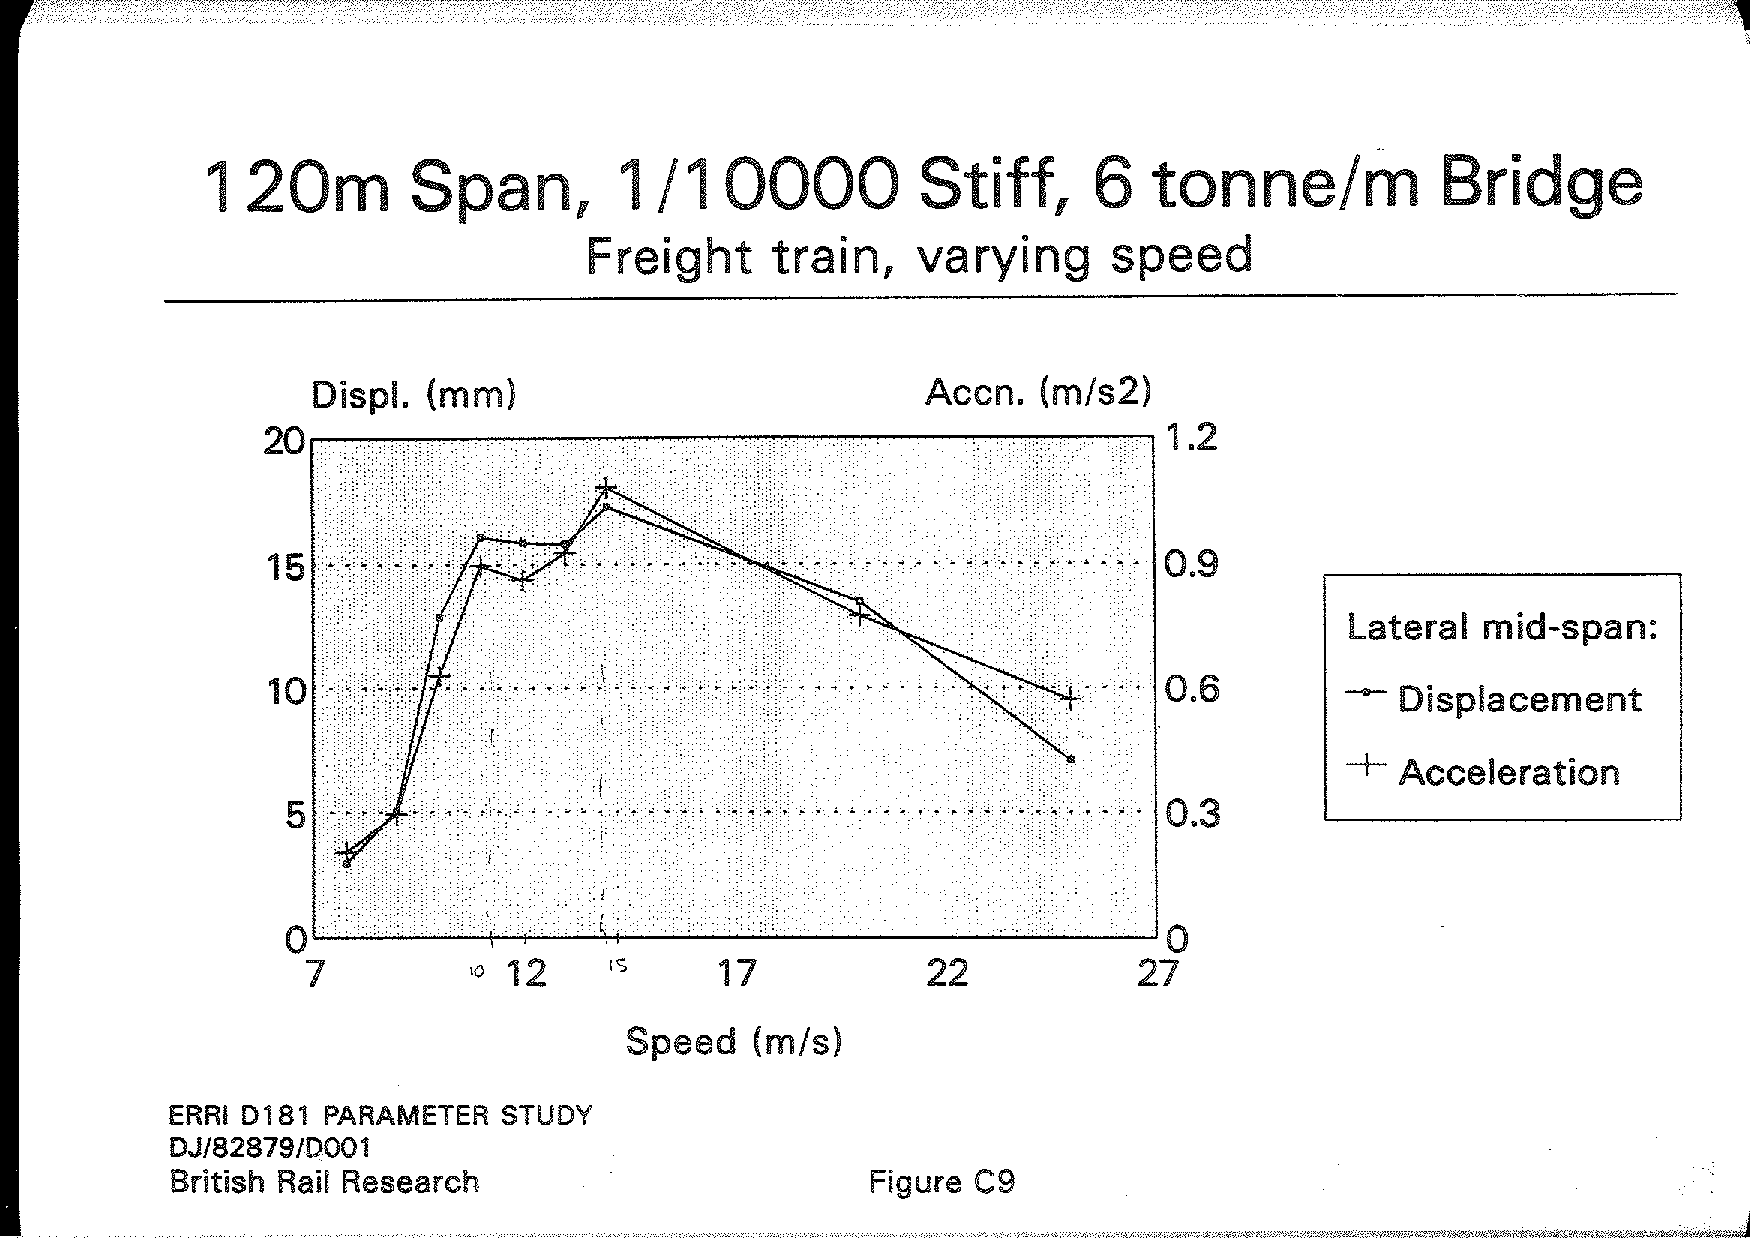
\includegraphics[height = 0.25\textheight]{c9}
    \caption{Figure C9 extracted from \citet{d181dt329} }
    \label{fig:c9}
\end{figure}

Figure.\ref{fig:c9} illustrates a chosen simulation case. The bridge possesses following parameters:

$$
\begin{array}{c}
l = 120m \\ 
Stiff\footnotemark: \sfrac{1}{10000} \\ 
\mu = 6000kg/m\\
\end{array}
$$
\footnotetext{defleciton/span ratio at midspan under 100kN point load at midspan}

Peak result for numerical simulation: 17mm

According to the definition, the characteristic value of the nosing force shall be taken as $Q_{sk} = 100kN$. It shall not be multiplied by the factor $\Phi$ or by the factor $f$. Thus, according to simple support Euler-beam theory, the deflection under 100kN nosing force is:

$$\delta_{nosing} = 120m \cdot \sfrac{1}{10000} = 0.012m = 12mm$$

It can be seen that nosing force does not give conservative result compared to numerical simulations. The reason for the nonconservative result is that this simulation case reproduced vehicle-bridge resonance so the peak displacement is amplified. It can be concluded that nosing force in Eurocode does not take resonance effects into account. It is nonconservative when resonance between vehicle and bridge happens.

\section{Conclusion}
According to the analysis, the Eurocode criterion based on bridge natural frequency lacks theoretical support thus no principle can be extracted from this criterion. The resonance type described in the criterion is not validated by any research and the criterion can not avoid any known resonance type. 

The criterion based on lateral forces is feasible but too conservative in original proposal because nowadays tracks and wheels are well maintained so lateral forces on tracks are much smaller than those generated from UIC simulations. However, nosing force in Eurocode is reduced in magnitude due to unknown reasons and the reduction may result in nonconservative result when resonance happens.

Thus it can be concluded that Eurocode criteria on lateral dynamics of railway bridge lack adequate verification on resonance effects. 

Since the bridge of Iv-Infra can not meet bridge natural frequency based criterion and this criterion is intended to solve resonance issues, the bridge should be verified for its lateral resonance behavior. Since the Eurocode criterion does not make sense, alternative assessment method for lateral railway bridge resonance behavior needs to be applied on the bridge of Iv-Infra.

